\documentclass[12pt]{article}

\usepackage[margin=1in]{geometry}
\usepackage{amsmath}
\usepackage{graphicx}
\usepackage{float}
\usepackage{subfig}
\usepackage{url}
\usepackage{appendix}

\title{The Doppler Effect}
\author{Logan Cantin}
\date{\today}

\begin{document}

\maketitle

\section{Introduction}

\subsection{The Doppler Effect}

The Doppler effect is a common phenomenon where the frequency of a wave increases
or decreases because the source is moving relative to the observer. Examples of this phenomenon include
the change in pitch of a siren on a passing ambulance or the redshift that astronomers
observe in planets. The Doppler effect is caused by the wavelength being shortened or
extended by the movement of the wave's source. Figure \ref{fig:comparison} provides a visual representation
of the Doppler effect.

\begin{figure}[H]
	\centering
	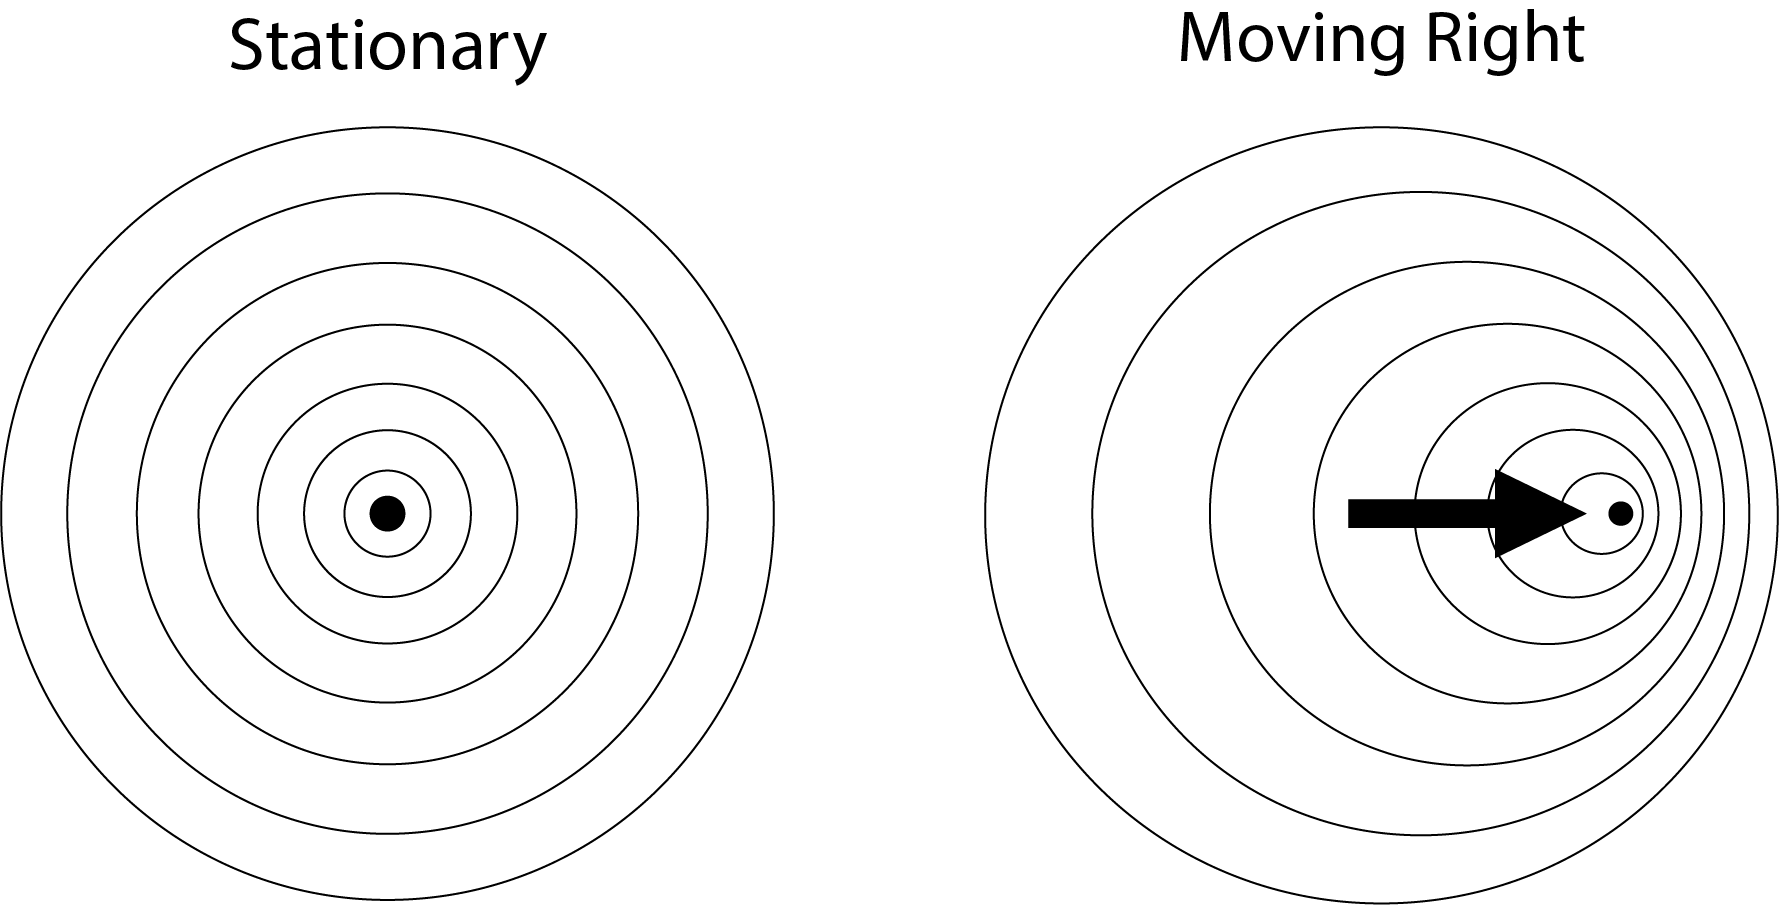
\includegraphics[width=5in]{comparison}
	\caption{Comparison of a stationary and moving source}
	\label{fig:comparison}
\end{figure}

It is possible to calculate the effective frequency of a wave affected by the Doppler effect.
The factors that affect it are the speed of sound in air ( $ v_a = 343 \text{ m/s}  $ ),
the frequency of the source ($ f_s $), and the speed of the source towards the observer 
($ v \text{s} $). Figure \ref{fig:wavelength} shows the difference between a wave with a stationary and 
moving source. Point A has travelled $ \lambda $ meters, and the source has 
travelled $0$ meters, resulting in a wavelength of $ \lambda _e = \lambda - 0 $ meters,
where $ \lambda _e $ is the effective wavelength due to the Doppler effect.
In contrast, Point B has travelled $ \lambda $ meters, but the source has travelled 
$ \frac{v_s}{f_s} $ meters, resulting in a new wavelength of $$ \lambda _e =  \lambda - \frac{v_s}{f_s} $$

\begin{figure}[H]
	\centering
	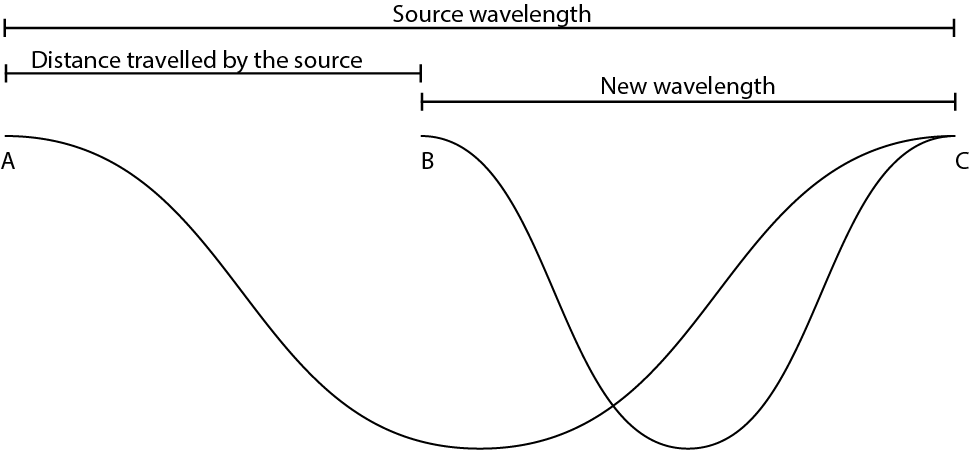
\includegraphics[width=5in]{wavelength}
	\caption{Illustration demonstrating why the Doppler effect takes place}
	\label{fig:wavelength}
\end{figure}

From here it is easy to calculate the effective frequency. Given that $f = \frac{v_a}{ \lambda } $, the effective wavelength can be substituded in and simplified, resulting in:
$$ f_e = \frac{f_s \cdot v_a}{ v_a - v_s }$$

The above formula works well when you're calculating the frequency one time. For reasons explained in Appendix A, this is not a good solution for modelling the frequency of a passing car. For this, we use

$$f(t) = f_0 \left( \frac{v_s}{v_s - v(t)} \right) $$

where $v(t)$ is

$$ v(t) = \frac{- (v_0)^2 t}{\sqrt{(v_0 t) ^ 2 + (d_0) ^ 2}} $$

$v_s$ is the speed of sound, $v_0$ is the speed of the car relative to the ground, and $d_0$ is the closest that the car and the observer are ever together. For a more complete explanation, refer to Appendix A.


\subsection{Analyzing Frequencies}

\begin{figure}[H]
	\centering
	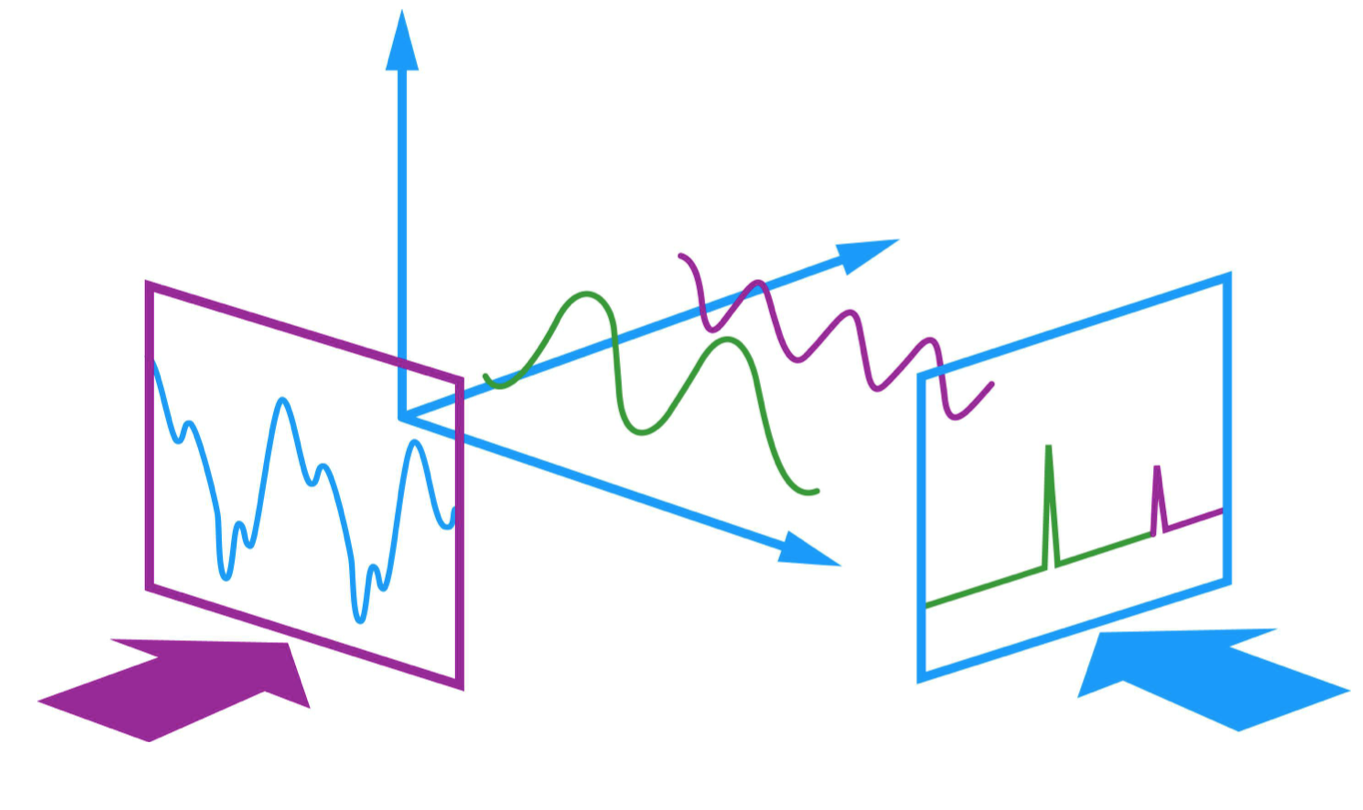
\includegraphics[width=5in]{composition}
	\caption{Visual intuition of the Fourier Transform}
	\label{fig:composition}
\end{figure}

All complex signals can be represented by the addition of many simple sine waves of different frequencies and magnitudes. This discovery was made by Joseph Fourier and is known as the Fourier Transform. Figure \ref{fig:composition}
shows an example of a complex signal, the waves that make it up, and its Fourier Transform. Simply put, the Fourier Transform determines the different frequencies that make up a complex signal
Sound waves can be analyzed with this method. Fields such as music, sonar, and speech
processing use these tools to analyze sound data. A common tool for analyzing sound
data is the spectrogram. Figure \ref{fig:spectrogram} shows an example of what a spectrogram looks like. The x axis is frequency, and the y axis is time. 
A custom spectrogram that I programmed will be used to analyze the sound data recorded for this lab.

\begin{figure}[H]
	\centering
	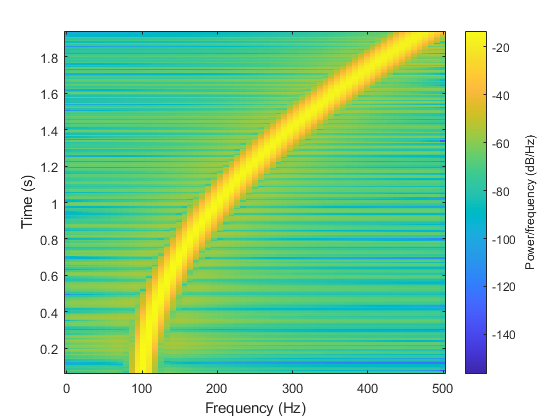
\includegraphics[width=5in]{spectrogram}
	\caption{The spectrogram of a tone starting at 100Hz and increasing 500Hz in 2 seconds. }
	\label{fig:spectrogram}
\end{figure}


\section{Hypothesis}
The hypothesis that this lab will attempt to prove is that the formula 
$$ f(t) = \frac{f_s \cdot v_s}{ v_s - v(t) }$$ 
is an accurate representation of the frequency of a wave affected by the Doppler effect. 

\section{Method}
\subsection{Apparatus}

\begin{itemize}
    \item Speaker
    \item Car
    \item Tone generator
    \item 2 Sound recorders
\end{itemize}

\subsection{Procedure}

\begin{enumerate}
    \item A quiet road was found. The speaker was attached to the tone generator and
    was placed in the car. The windows were rolled down. The sound recording device
    was held at the side of the road.
    \item For each speed (60km/h, 75km/h, 90km/h), a tone of 300, 500, 700 and 900Hz were each played one at a time and recorded using the sound recorder.
    
    \item Each of the audio files were converted to the .wav format.
    \item The audio files were then analyzed with the spectrogram.
    \item The theoretical frequency was calculated using the formula $$ f(t) = \frac{f_s \cdot v_s}{ v_s - v(t) }$$
    \item The audio file was shifted left or right so that the time that the car passed was 0 seconds in the graph.
\end{enumerate}

\section{Results and analysis}

The following graphs show the actual frequency of tone as it passes (red x's) compared to the theoretical values (red line). A larger version is available in the Appendix. The rows all contain the same frequency (300, 500, 700, and 900Hz) and the columns are the different speeds (60, 75, and 90km/h).

\subsection{Observations}

\begin{figure}[H]
	\centering
	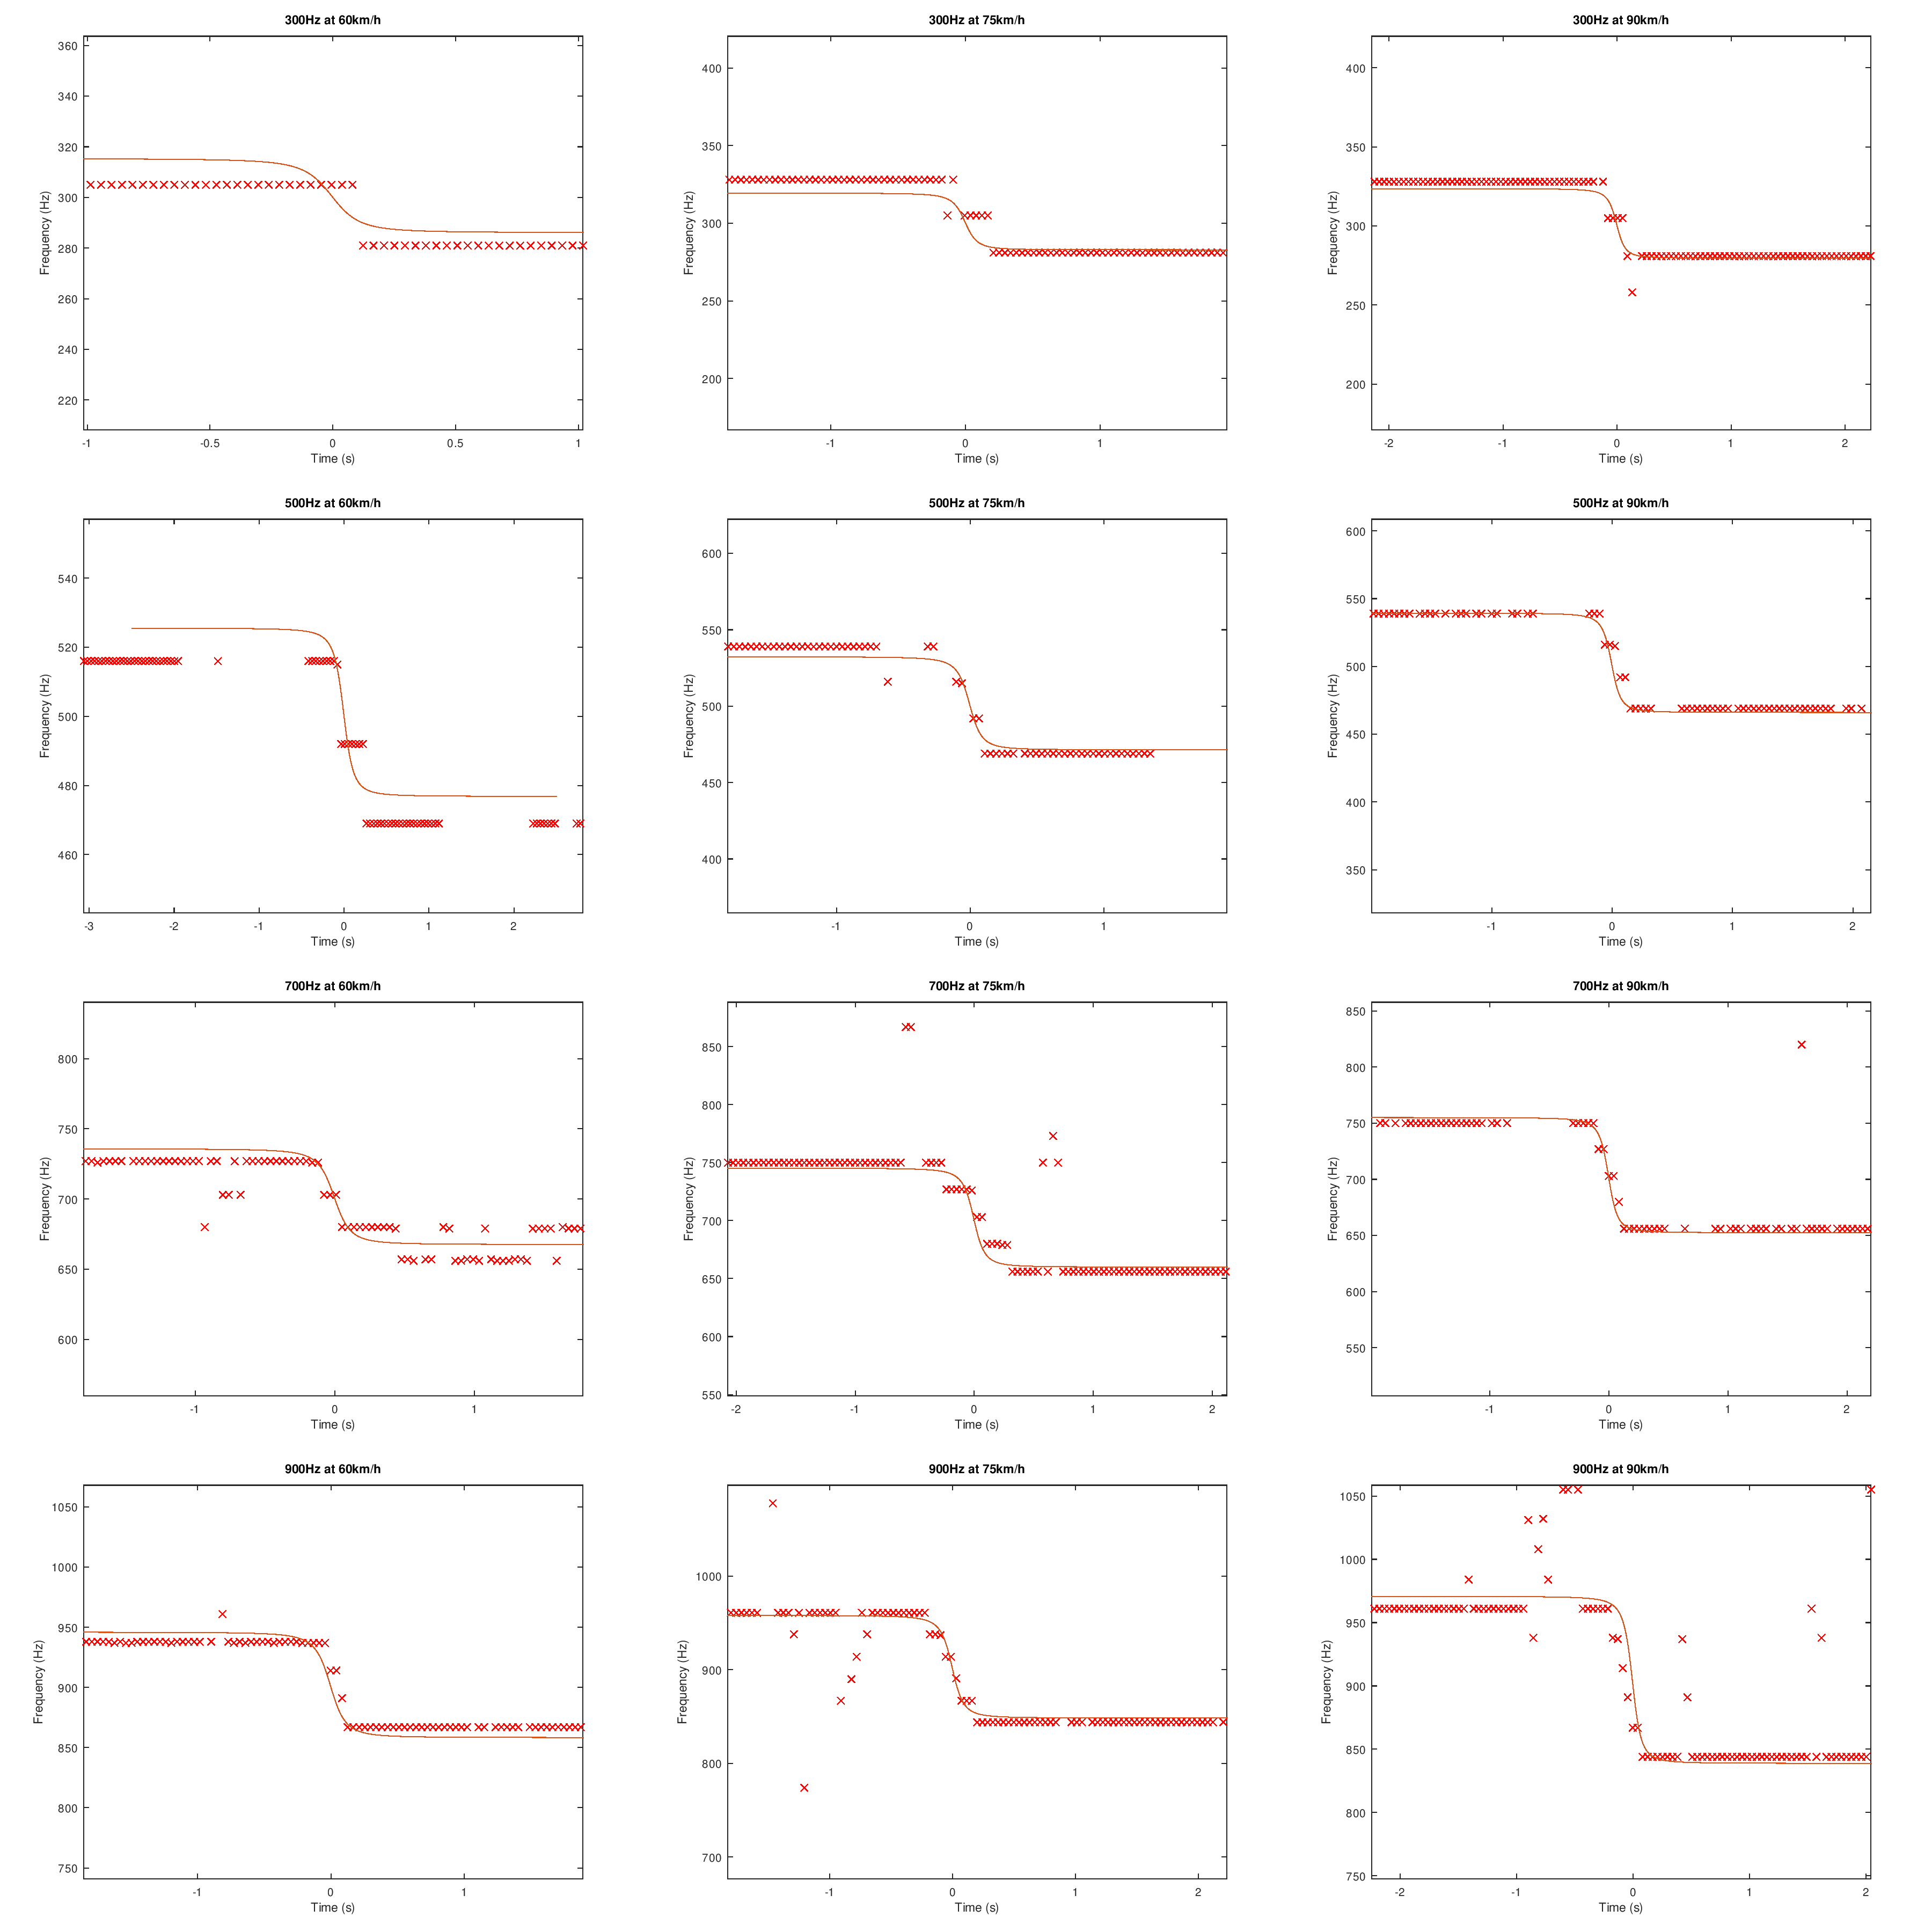
\includegraphics[width=7in]{resultsvert}
	\caption{Results}
	\label{fig:results}
\end{figure}

\subsection{Sources of error}

The main sources of error are:

\begin{itemize}
\item \textbf{Noise.} The audio files contain noise other than the tone, which can skew the readings. Two examples of noise that caused significant issues were wind and other cars passing by. At slower speeds, there tended to be more noise. Noise presents itself in the graphs as data points in unexpected places and gaps in the data.
\item \textbf{Fourier Uncertainty Principle.} Due to the mathematical principles of the Fourier Transform, there is a fundamental trade-off between frequency and time accuracy, very similar to the Heisenberg Uncertainty Principle. That is, you can only get an accurate time or frequency measurement, but not both. In the context of this experiment, I had to sacrifice some frequency accuracy in order to get accurate timing information. It is for this reason that measured frequencies tend to be in particular rows and not continuous as would be expected. This effect is most prominent in the lower frequencies. This effect was mitigated by adding frequency interpolation.
\item \textbf{Simplification.} In order to reduce visual clutter, I opted to forego the full spectrogram in favour of a simplified version. The simplified version that is visible in the observation charts takes the most powerful frequency at each time sample. Noise and other sounds can really skew the point that is generated on the final chart. By contrast, all the nuance is kept in a spectrometer and the tone can be visualized at all times, regardless of other noises.
\end{itemize}


\section{Discussion}
The hypothesis was proven to be correct to an accuracy of $\pm$ 10Hz. In some cases, the hypothesis was exactly correct.

This section will explain the characteristic 'swoop' of the Doppler effect and discuss the practical implications and interesting phenomena that are a result of the Doppler effect.


\subsubsection{Swoop}
The characteristic sound of the Doppler effect comes from the "swoop" that is heard as the source passes the observer. This smooth swoop is a result of the distance that exists between the source and the observer. To illustrate my point, lets substitute $d_0 = 0$ into $v(t)$ (Figure \ref{fig:zero}). What you will notice is that the velocity remains the same for all negative time values, and then abruptly jumps to the negative for all positive time values. In this case, the source is literally passing directly through the observer. 

\begin{figure}[H]
	\centering
	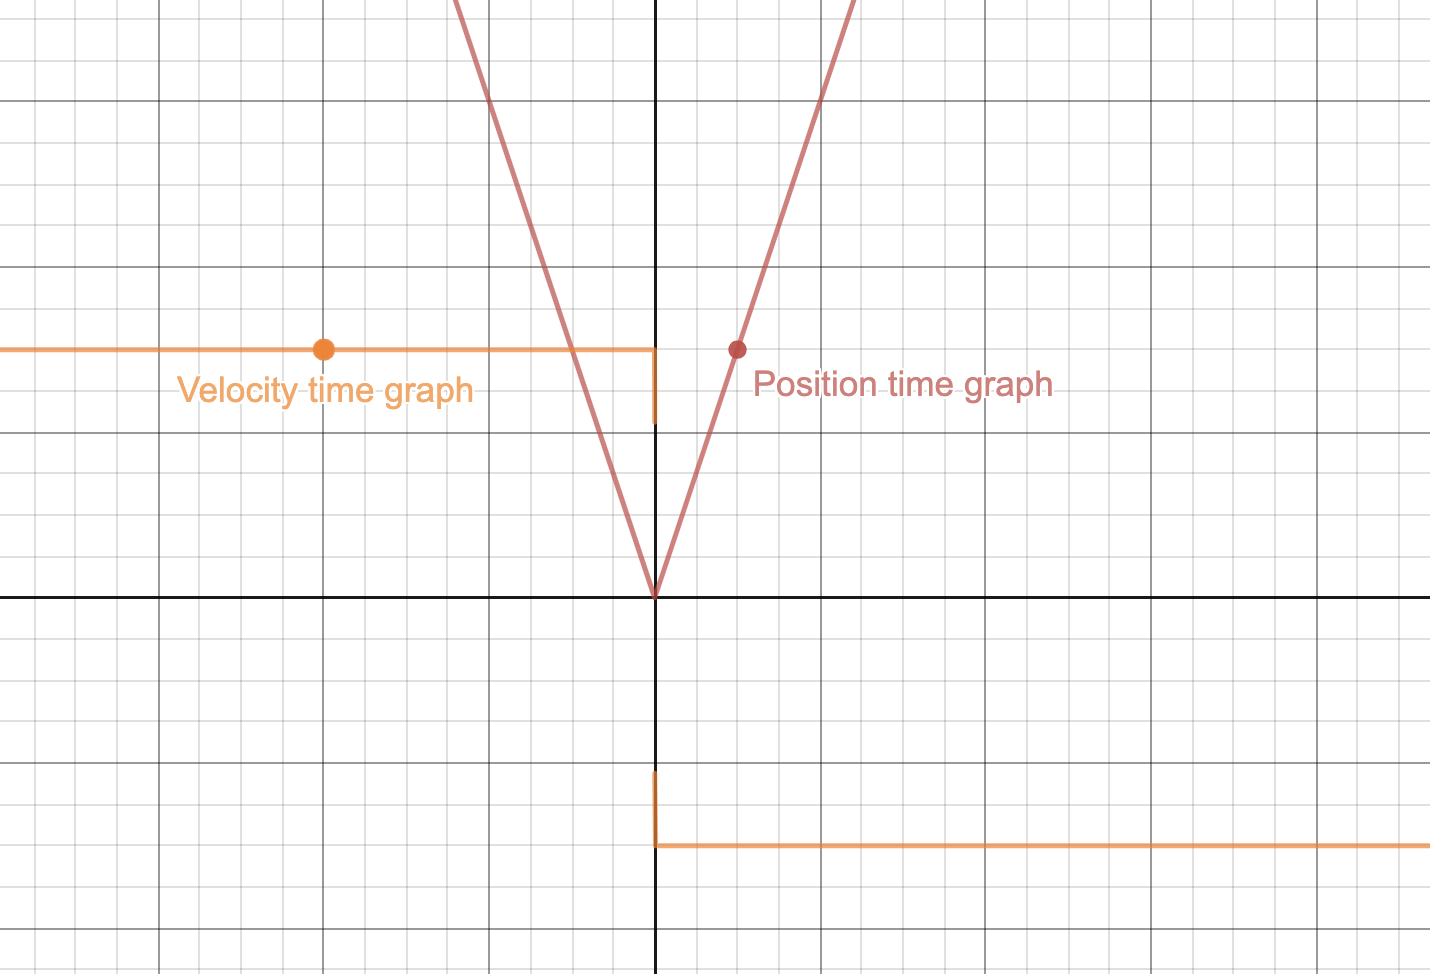
\includegraphics[width=5in]{zerodistance}
	\caption{Position and velocity graphs when $d=0$}
	\label{fig:zero}
\end{figure}

Since this is not possible in real scenarios, there is always a positive distance between the source and the observer, in other words $d_0 > 0$. Because of this the velocity, and by extension the frequency, gradually transition from $-v_0$ to $+v_0$. This transition is what causes the swoop. The smaller the $d_0$, the faster the swoop occurs.

\begin{figure}[H]
  \centering
  \subfloat[Small $d_0$]{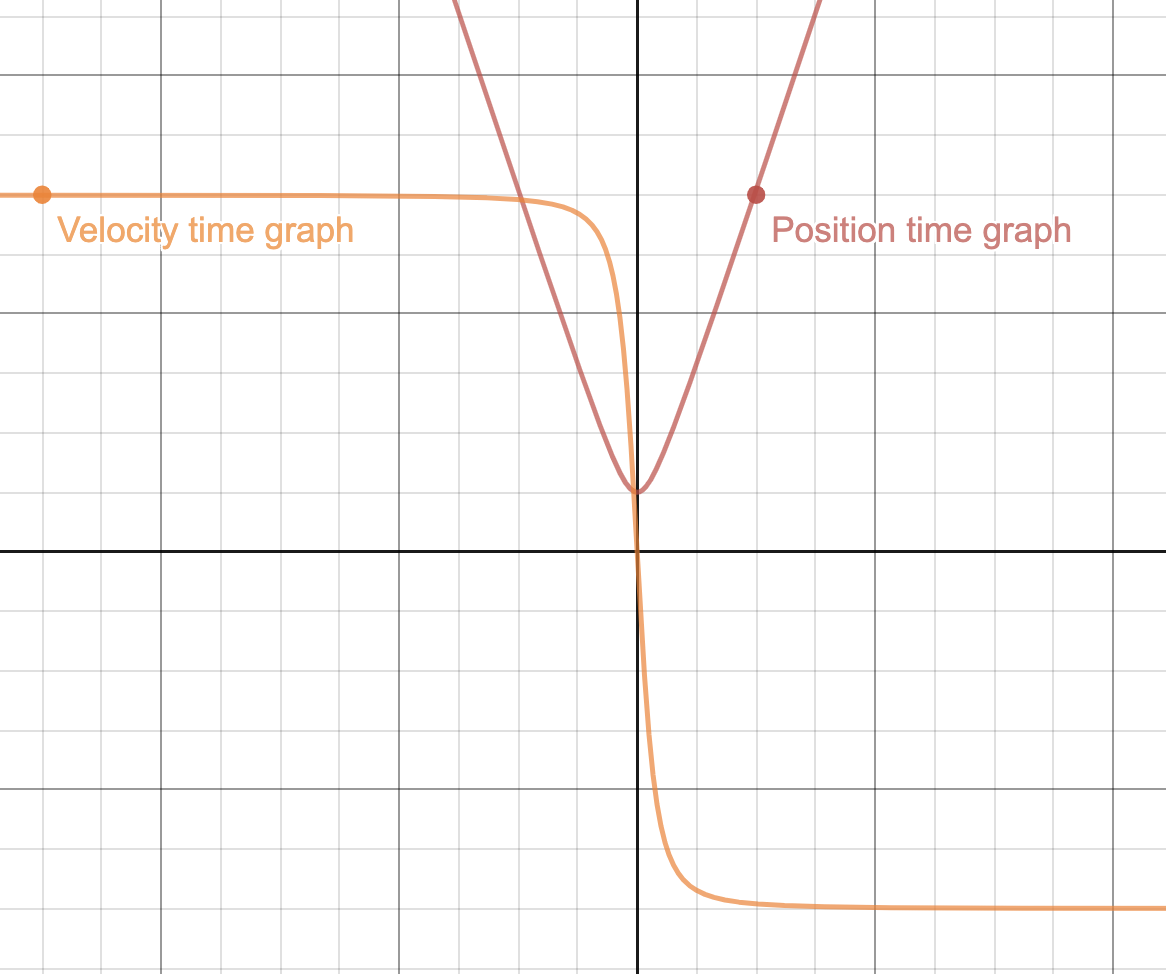
\includegraphics[width=0.4\textwidth]{smalld}\label{fig:smalld}}
  \hfill
  \subfloat[Large $d_0$]{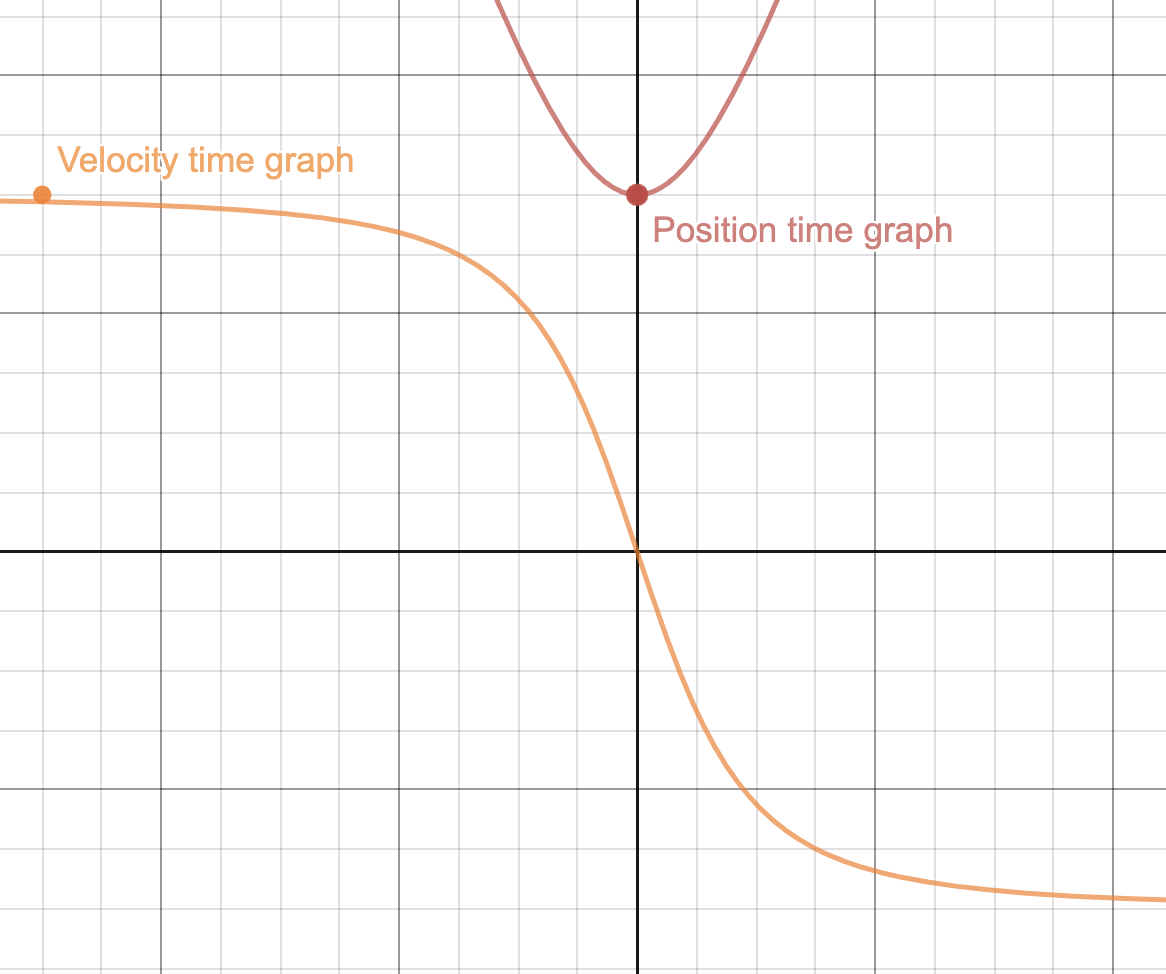
\includegraphics[width=0.4\textwidth]{bigd}\label{fig:bigd}}
  \caption{How $d_0$ affects the "swoop".}
\end{figure}

\subsubsection{Comparison between the new and old formulas}
Practically, the old formula is the new formula with $d_0 = 0$. This means that both formulas will yield similar results in the extremes, but the old formula lacks the smooth transition that the new formula has. Figure \ref{fig:zero} is an example of a graph with $d_0 = 0$, and Figure \ref{fig:smalld} and \ref{fig:bigd} show examples of graphs with $d_0 > 0$.

\subsection{Breaking the sound barrier}

The sound barrier, also known as the sonic barrier, is the sudden increase in aerodynamic drag and other undesirable consequences as a vehicule approaches the speed of sound (approximately 343 m/s or 1234 km/h, also know as Mach 1). The sound barrier caused many issues to pilots of high speed fighter jets in the Second World War, including numerous casualties. Today, many vehicles can break the sound barrier, including planes and even the Thrust SSC, the only car ever recorded to have gone faster than the speed of sound. Whips and most modern guns also break the sound barrier.

\begin{figure}[H]
	\centering
	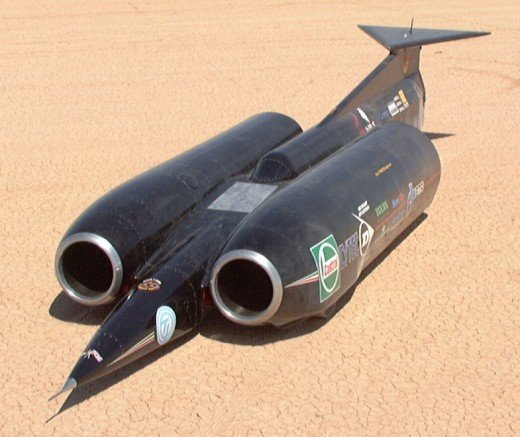
\includegraphics[width=2in]{thrust_ssc}
	\caption{The Thrust SSC, the only land vehicle to break the sound barrier}
	\label{fig:thrust}
\end{figure}

The sound barrier can be explained using the Doppler effect. As the speed of the source approaches the speed of sound (as shown in Figure \ref{fig:soundbarrier}), the observed frequency approaches infinity. Higher frequencies have higher pressure than lower frequencies, so the pressures of the increasing frequencies add together to make a wall of pressure which resists further acceleration past the speed of sound. At the speed of sound, the sound waves produced by the vehicle are moving at the same speed as the vehicle, causing turbulence and making this a very unsafe speed to be travelling at. This is also the time when the aerodynamic drag is at its peak. At speeds above Mach 1, the drag is greatly reduced as all of the sound waves created by the vehicle get left behind it. Anybody in front of a vehicle travelling above Mach 1 will not be able to hear it approach. 

\begin{figure}[H]
	\centering
	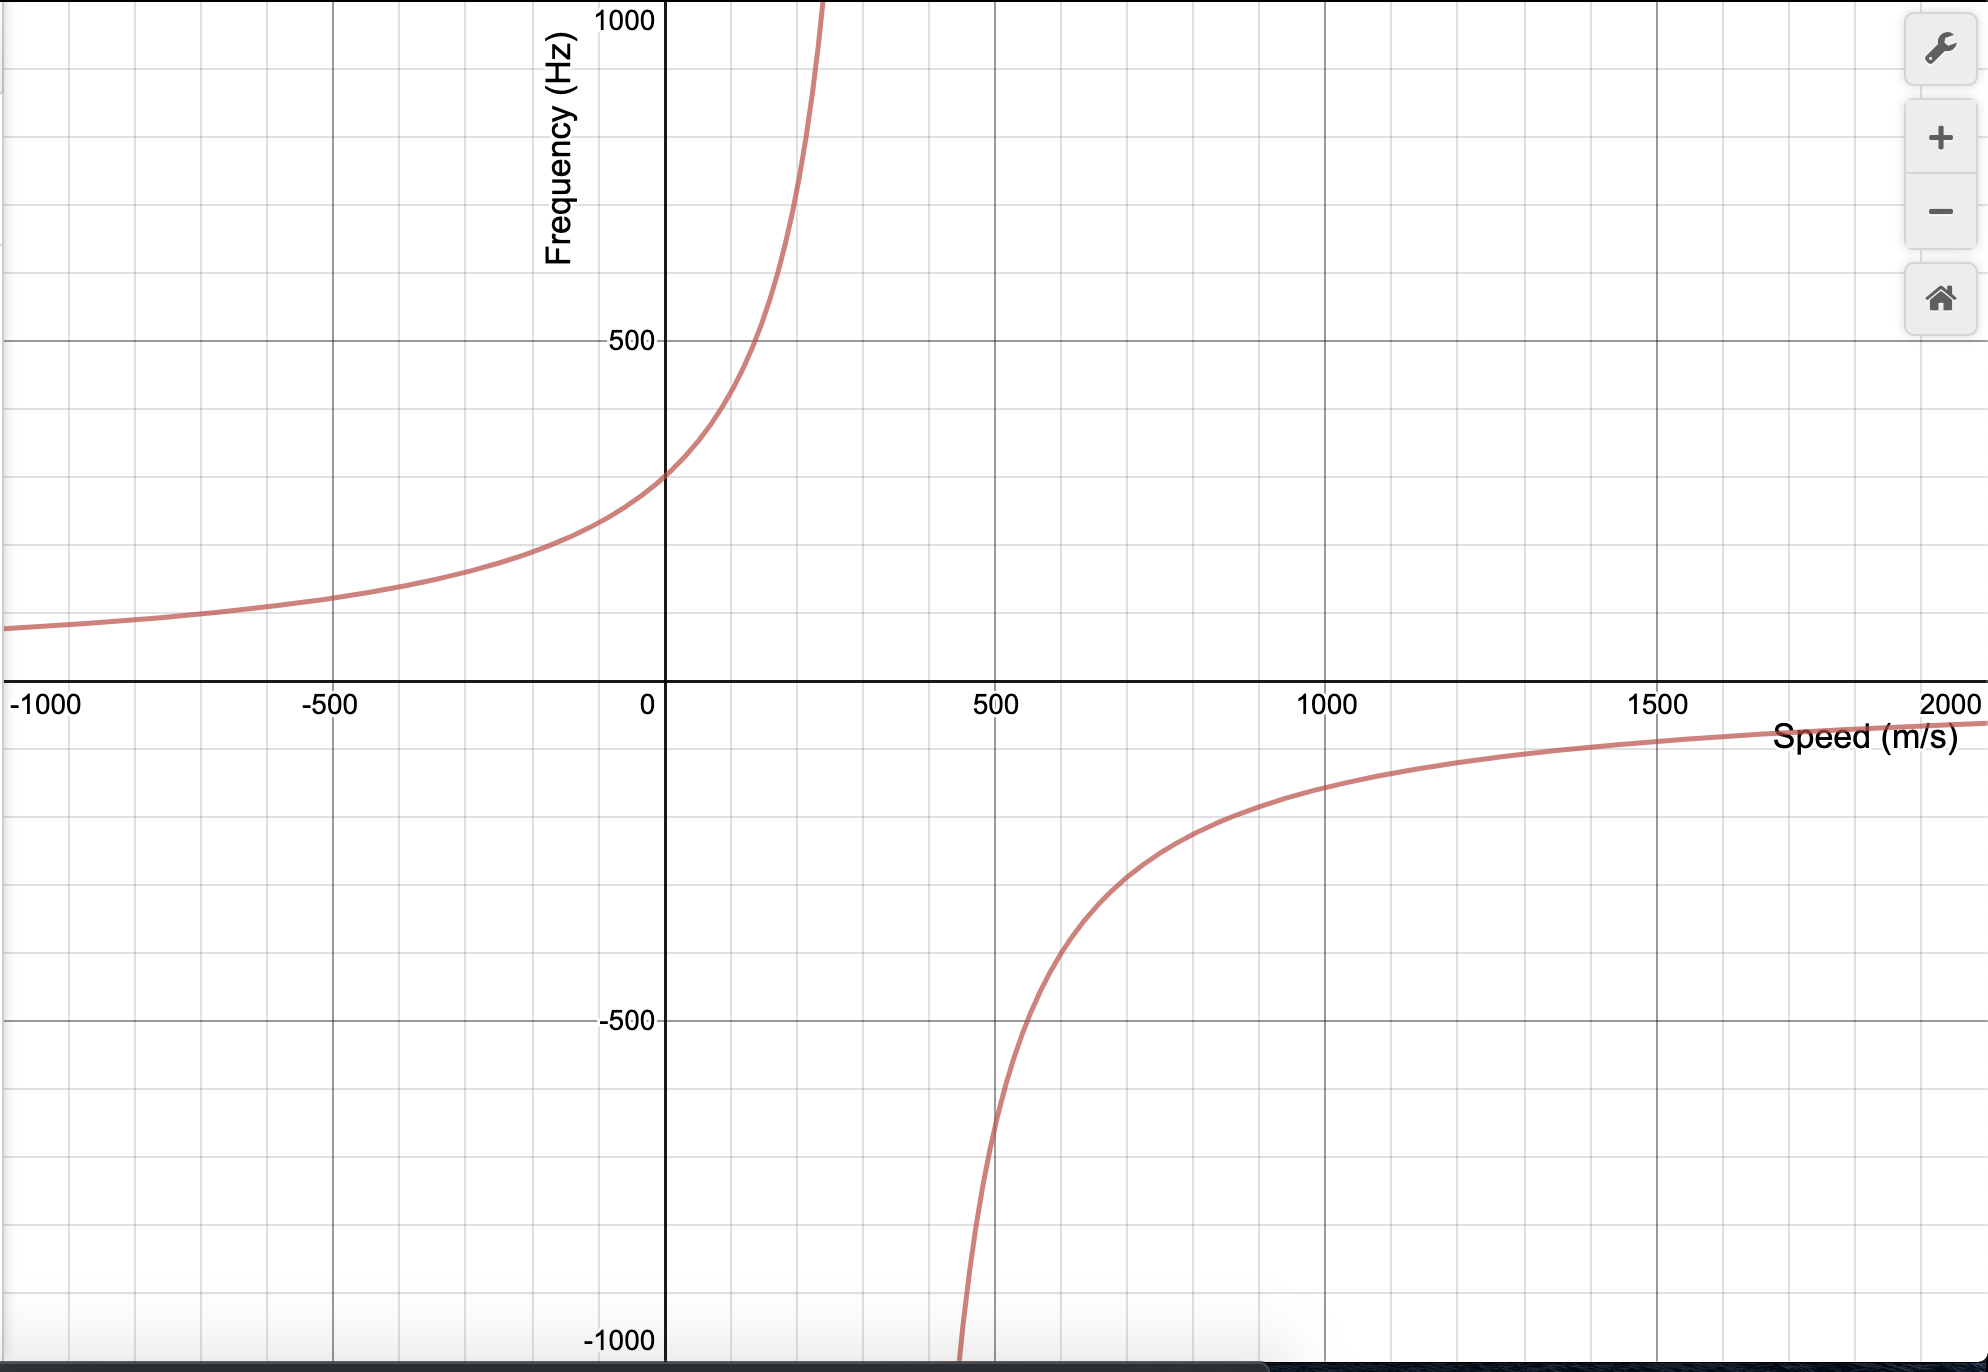
\includegraphics[width=5in]{soundbarrier}
	\caption{Observed frequency as vehicle accelerates towards Mach 1.}
	\label{fig:soundbarrier}
\end{figure}

\subsection{Cherenkov radiation and Redshift}

So far, only the applications of the Doppler effect on sound have been discussed. However, it also applies to light and other waves. This section will discuss how the Doppler effect is present in different phenomena relating to light.

\subsubsection{Redshift}

The discovery of redshift (also known as the Doppler-Fizeau effect) gave us some key insight into the nature of the universe and is also strong evidence of the Big Bang. Figure \ref{fig:redshift} demonstrates the redshift. Each star has a unique "signature", the absorption lines that are caused by the elements that make it up. Astronomers noticed that the absorption lines of elements on earth are different than what they observed when looking at stars. Using the principles given by the Doppler Effect, astronomers realized that the stars were all moving away from the Earth, which is what caused the unexpected shifting of the absorption lines. This realization supports the theory of the Big Bang and told scientists that the universe is expanding.

\begin{figure}[H]
	\centering
	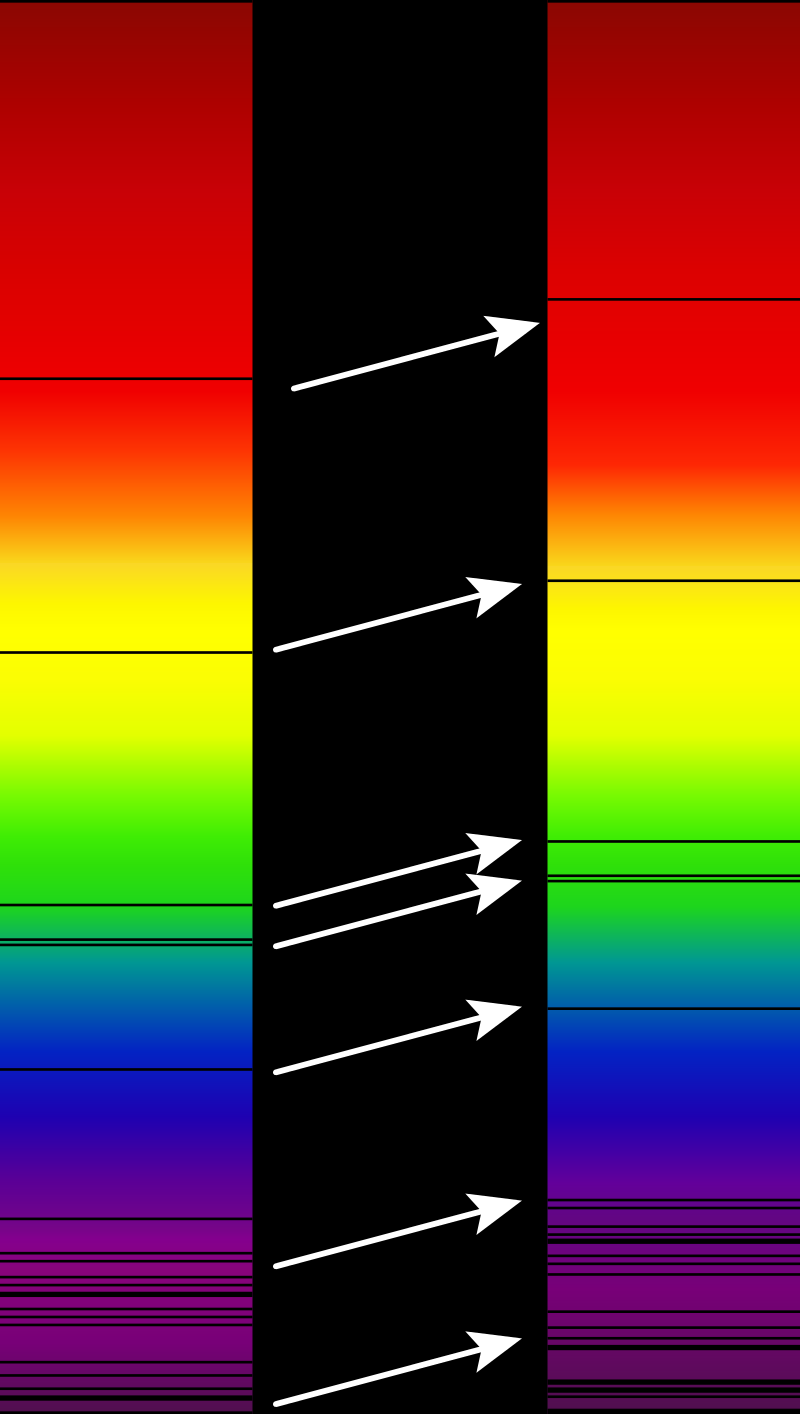
\includegraphics[width=2in]{redshift}
	\caption{The shifting of the absorption lines of a star that is moving away from the observer.}
	\label{fig:redshift}
\end{figure}

\subsubsection{Cherenkov Radiation}

Interestingly, the idea of a sonic boom doesn't only apply to sound. This may seem counter-intuitive, as the speed of light is the absolute speed limit in the universe. However, light travelling through mediums such as water or glass is significantly slower than the speed of light in a vacuum. This opens up the opportunity for other things to go faster than light.

In nuclear reactors that are submerged under water, the subatomic particles released by nuclear fission are launched at extremely high speeds. The speed of light in water is relatively slow, at only 75\% of the speed of light in a vacuum. These subatomic particles excite the matter they pass through and release photons, which causes the signature blue glow from nuclear reactors.

\begin{figure}[H]
	\centering
	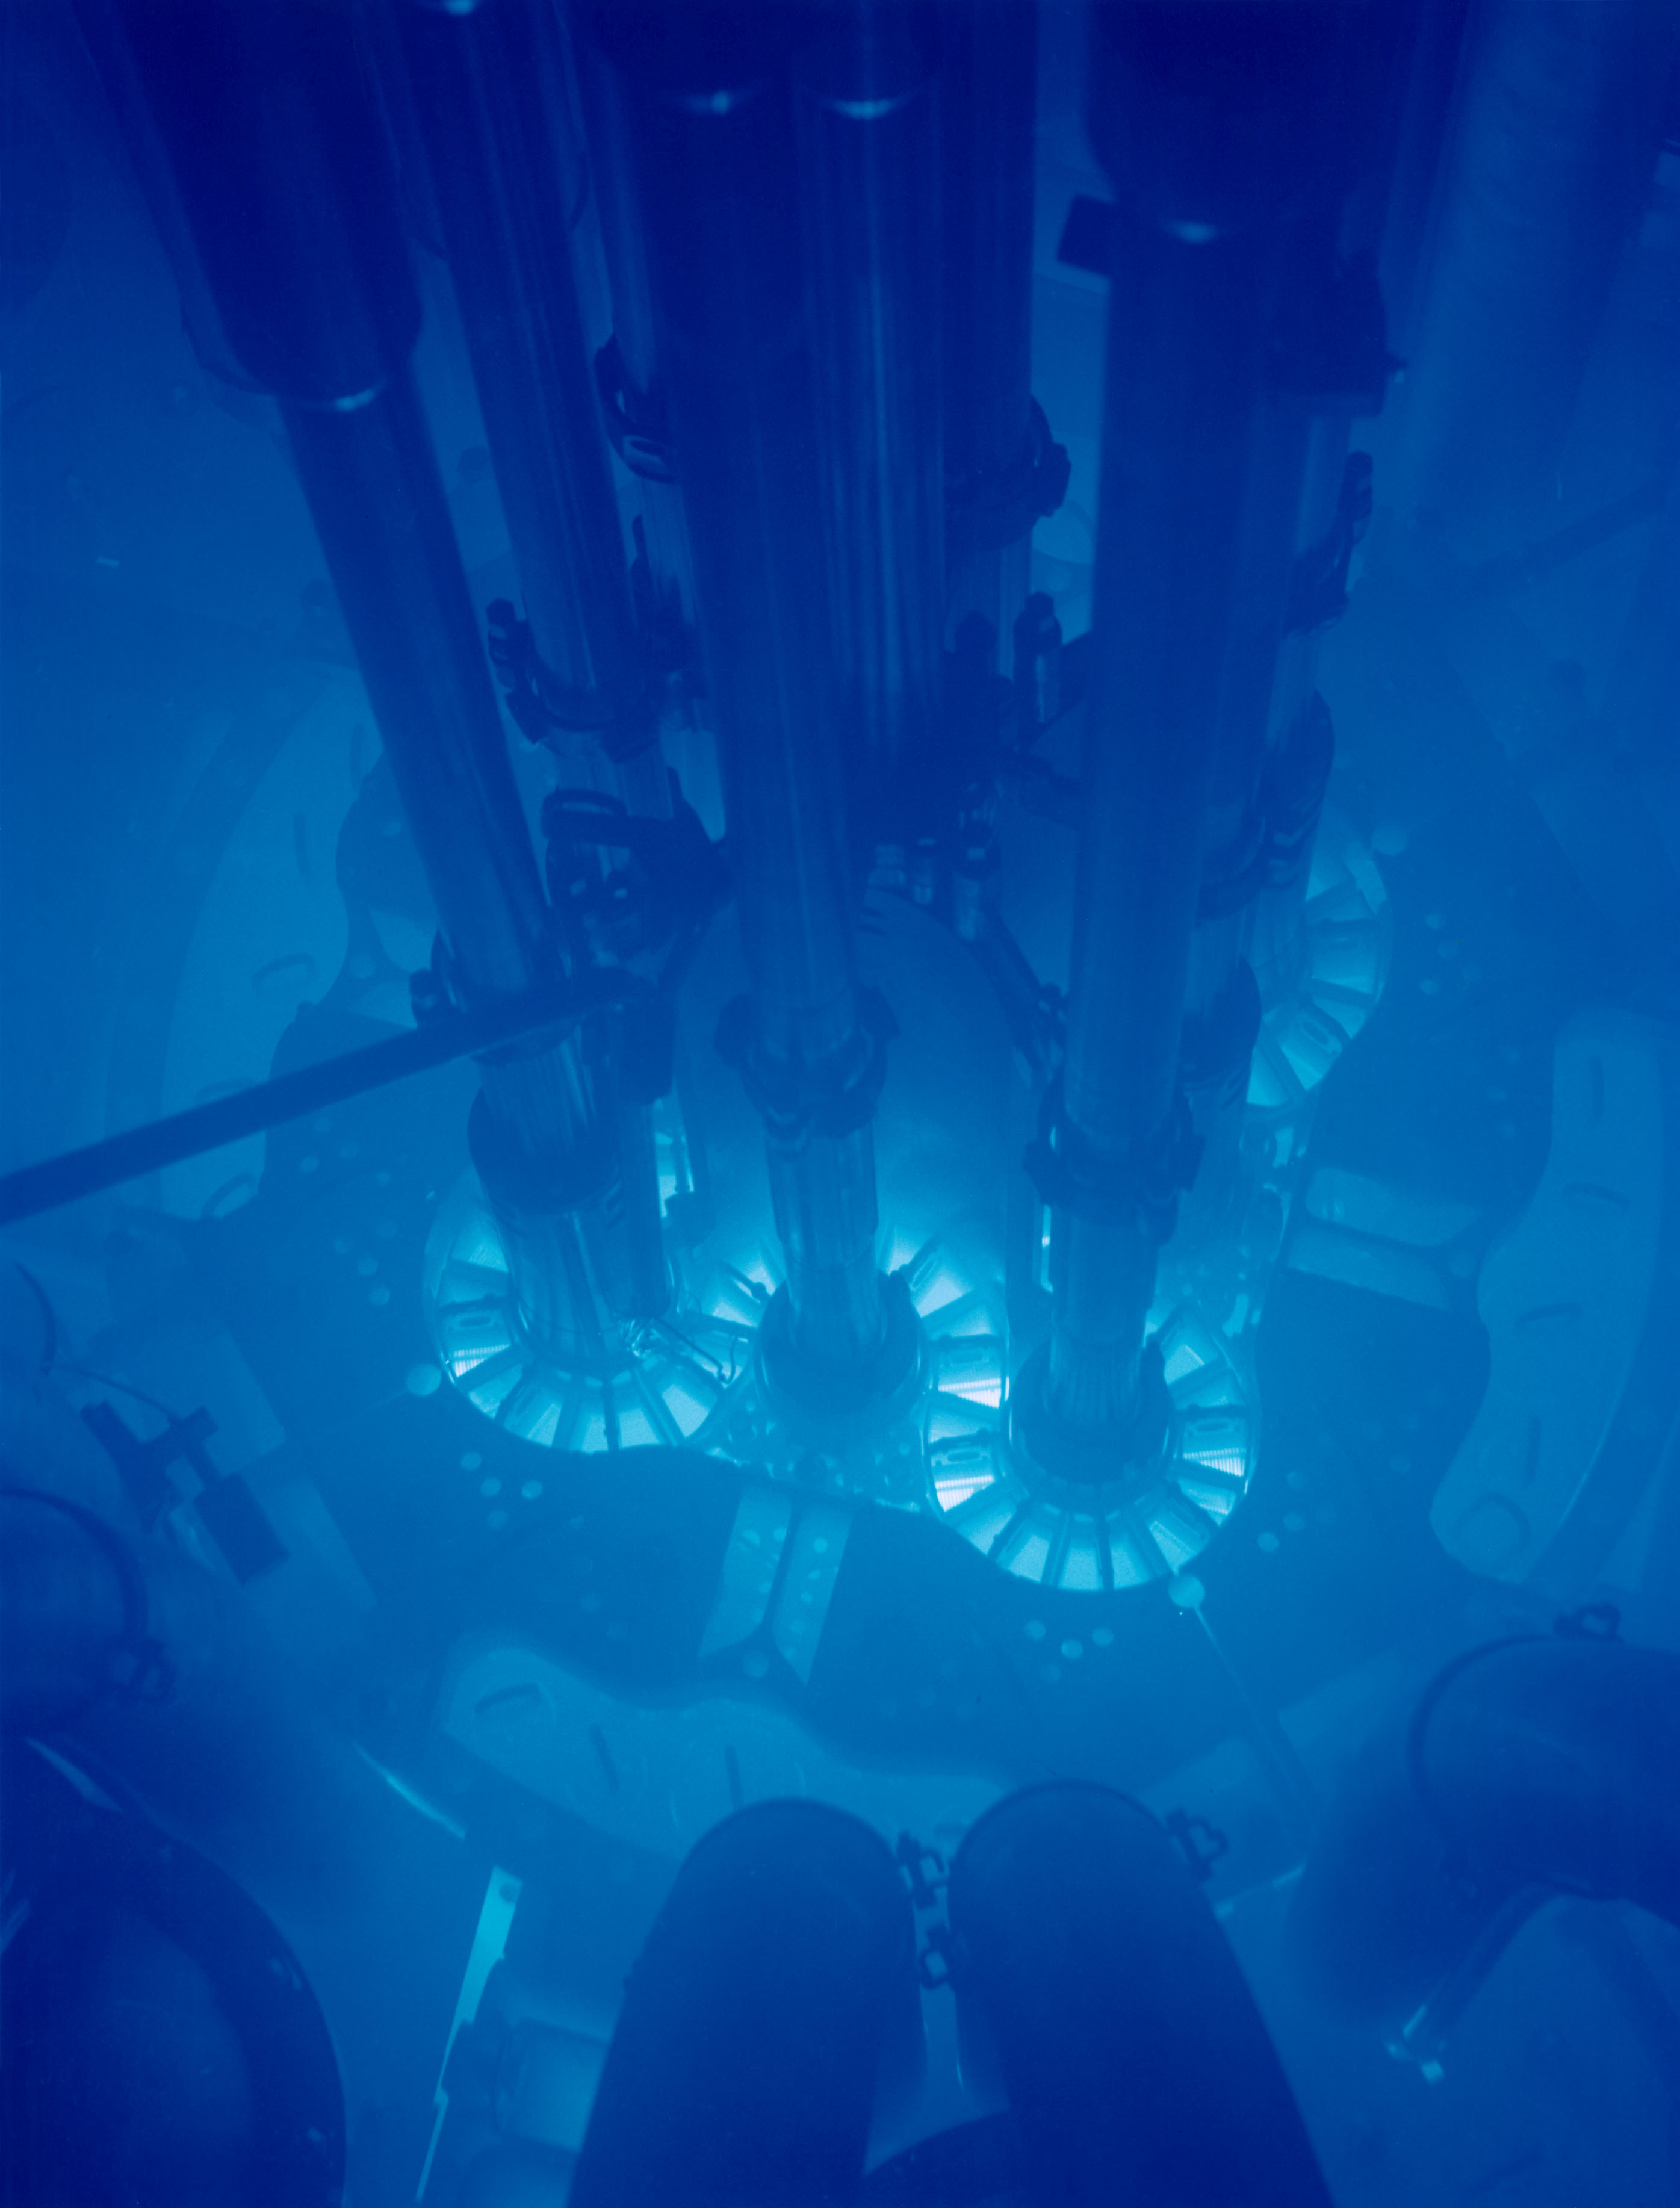
\includegraphics[width=4in]{reactor}
	\caption{Cherenkov radiation caused by a submerged nuclear reactor.}
	\label{fig:reactor}
\end{figure}

\section*{Appendix}

\appendix

\section{Deriving a more accurate formula}

The shortcoming of the original formula ($ f_e = \frac{f_s \cdot v_a}{ v_a - v_s }$) that was derived earlier in this report is that it relies solely on the speed of the source relative to the ground.  However, the speed that really matters  is the speed that the source is moving in the direction of the observer. The importance of this step becomes obvious in Figure \ref{fig:angle}, where the difference in frequency between observer A's perspective  and observer B's. 

\begin{figure}[H]
	\centering
	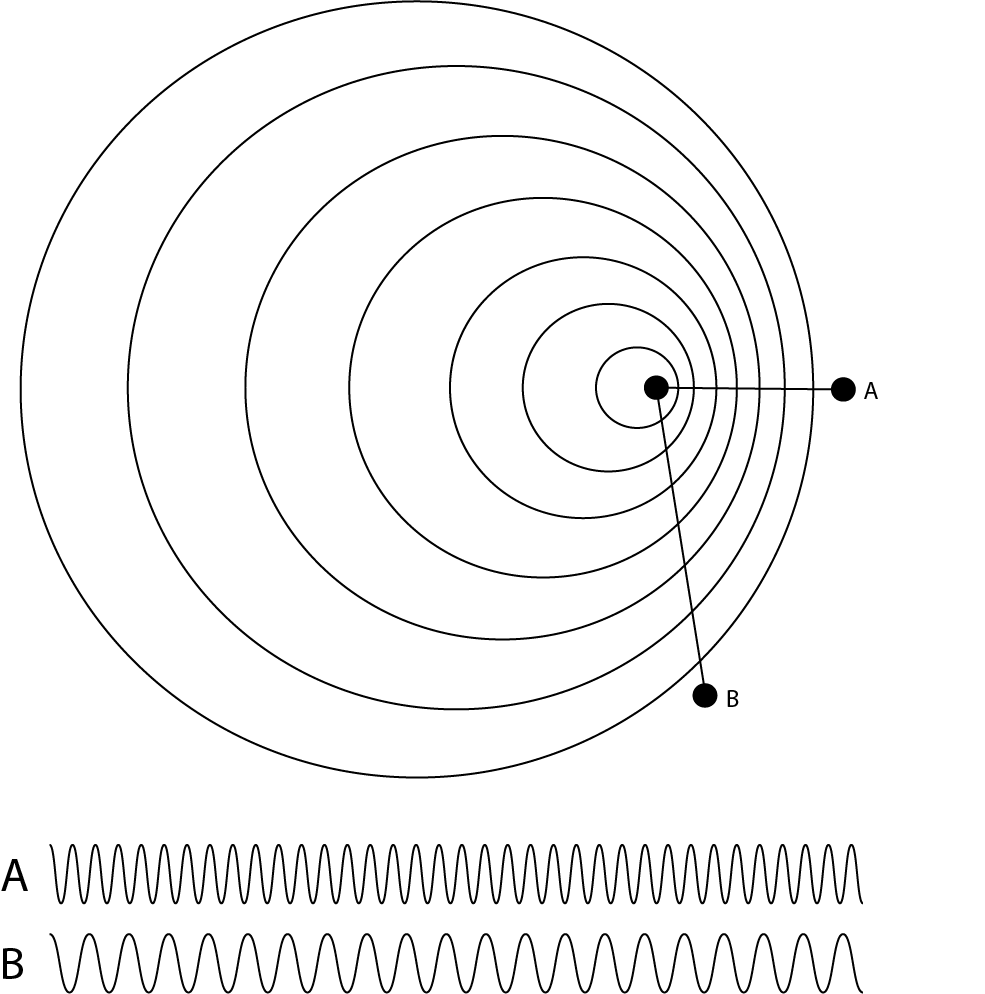
\includegraphics[width=5in]{angle}
	\caption{Demonstrating the importance of calculating the correct angle}
	\label{fig:angle}
\end{figure}

Since $ v = \frac{d}{t} $, the first step is finding the distance between the source and the observer at any given time.

\subsection{Distance between the source and the observer}

Given that the observer is at the origin and the source is moving in a straight line and at a constant speed $v_0$, the position of the source at any given time is $$ P(t) = (v_0 t, d_0)$$ where $d_0$ is the distance between the source and the observer when they are closest. Using the formula for Cartesian distance, we can determine that the distance between the source and the observer is $$ d(t) = \sqrt{(v_0 t) ^ 2 + (d_0) ^ 2} $$

\begin{figure}[H]
	\centering
	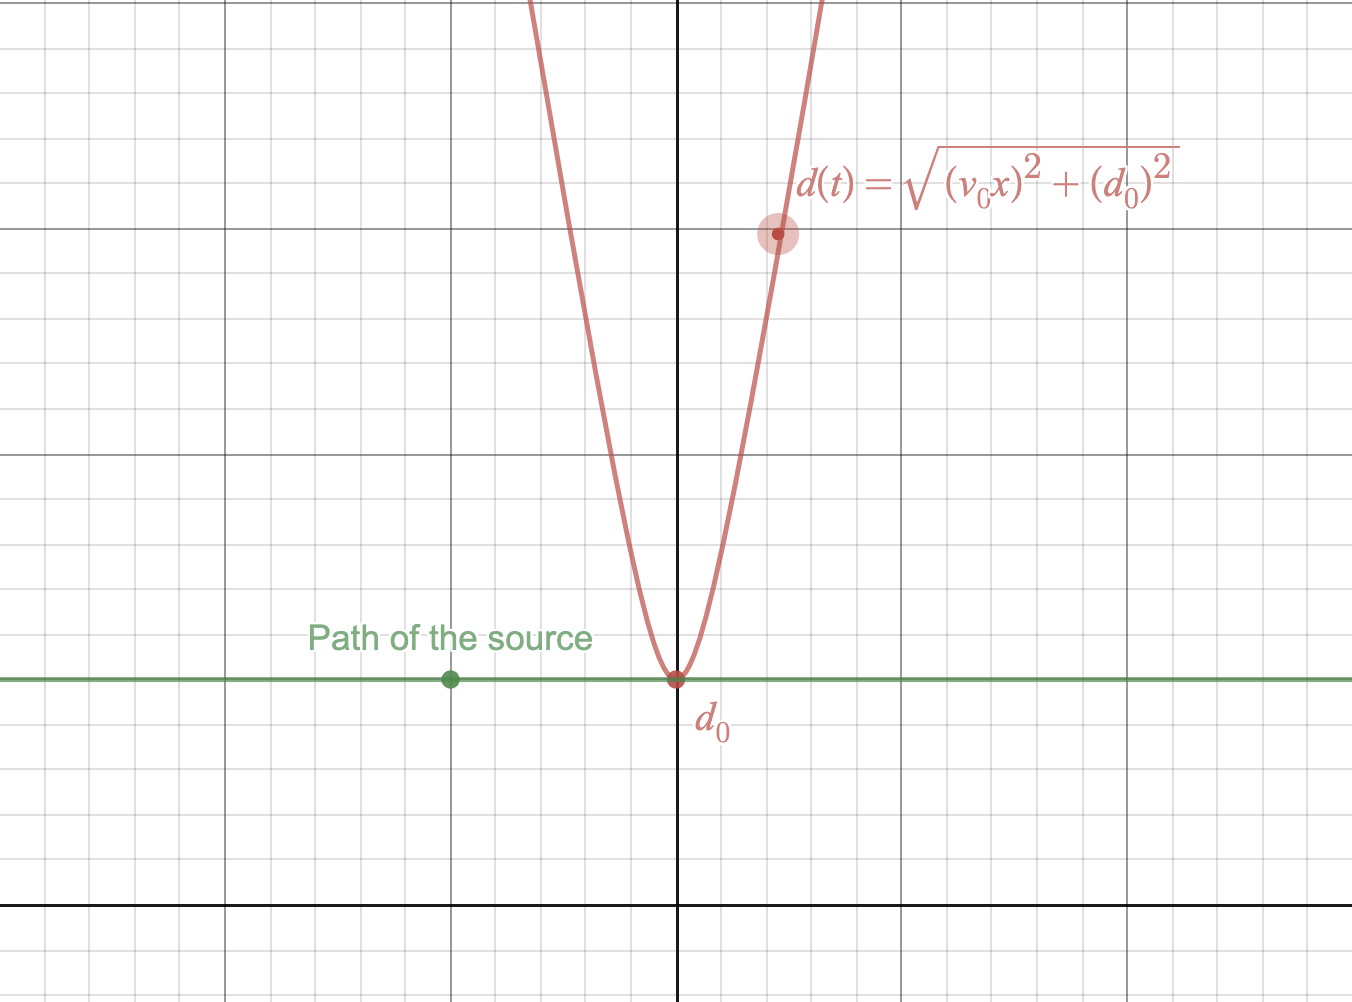
\includegraphics[width=5in]{distance}
	\caption{Graph showing the distance between the path and the source at a given time}
	\label{fig:distance}
\end{figure}

\subsection{Speed of the source in the direction of the observer}

Speed can be determined from the position time graph that was determined above by taking the first derivative. Therefore, the speed at time $t$ is $$ v(t) = \frac{- (v_0)^2 t}{\sqrt{(v_0 t) ^ 2 + (d_0) ^ 2}} $$

\begin{figure}[H]
	\centering
	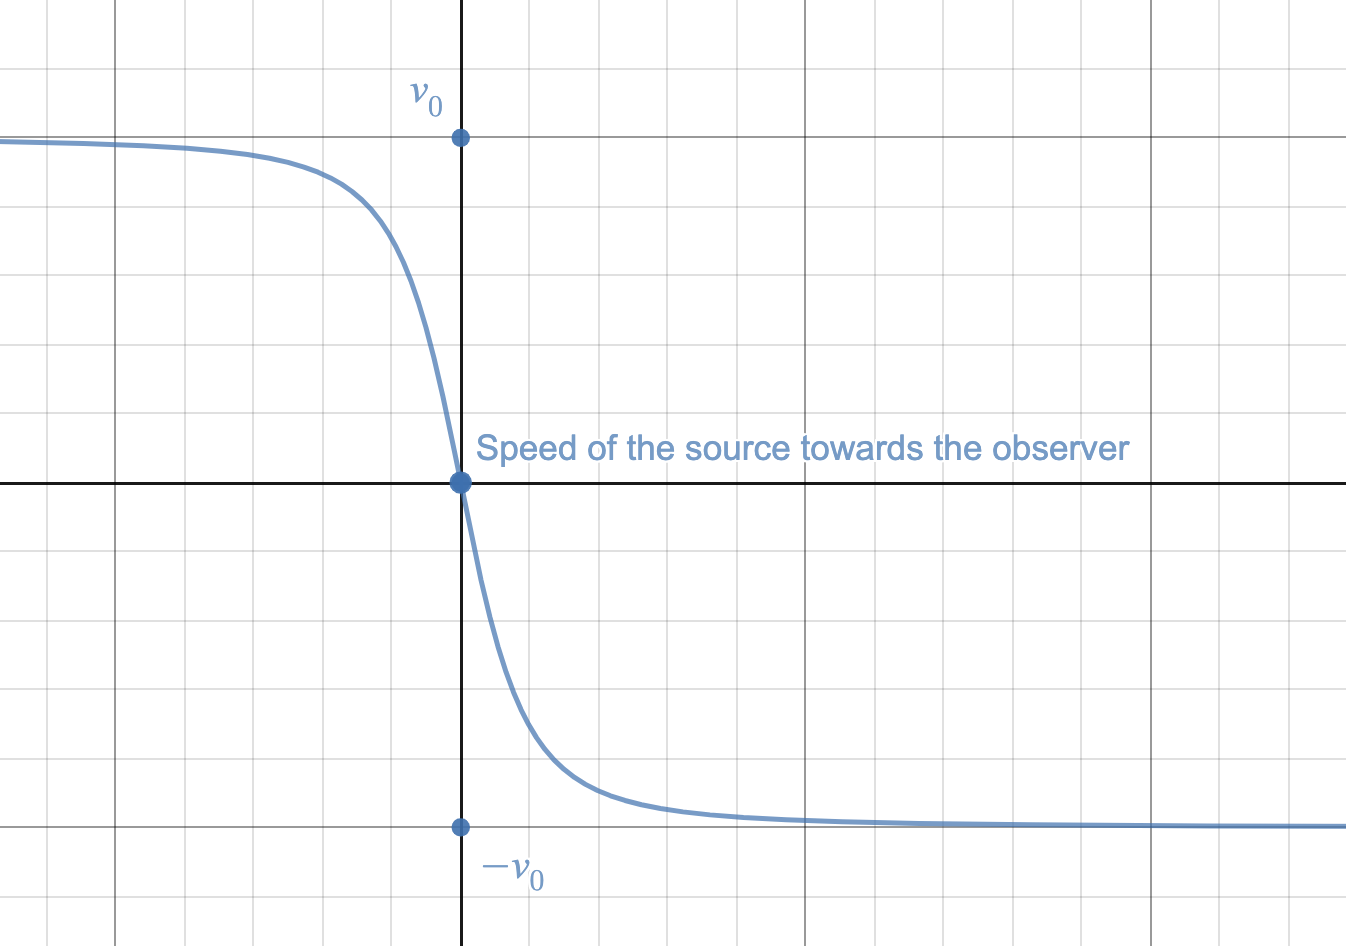
\includegraphics[width=5in]{velocity}
	\caption{Graph showing the speed of the source in the direction of the observer at a given time}
	\label{fig:velocity}
\end{figure}

\subsection{Observed Frequency}

Substituting our new equation for speed into the original formula for frequency, we can now get a more whole picture of the frequency that is heard by the observer at all times.  $$f(t) = f_0 \left( \frac{v_s}{v_s - v(t)} \right) $$

\begin{figure}[H]
	\centering
	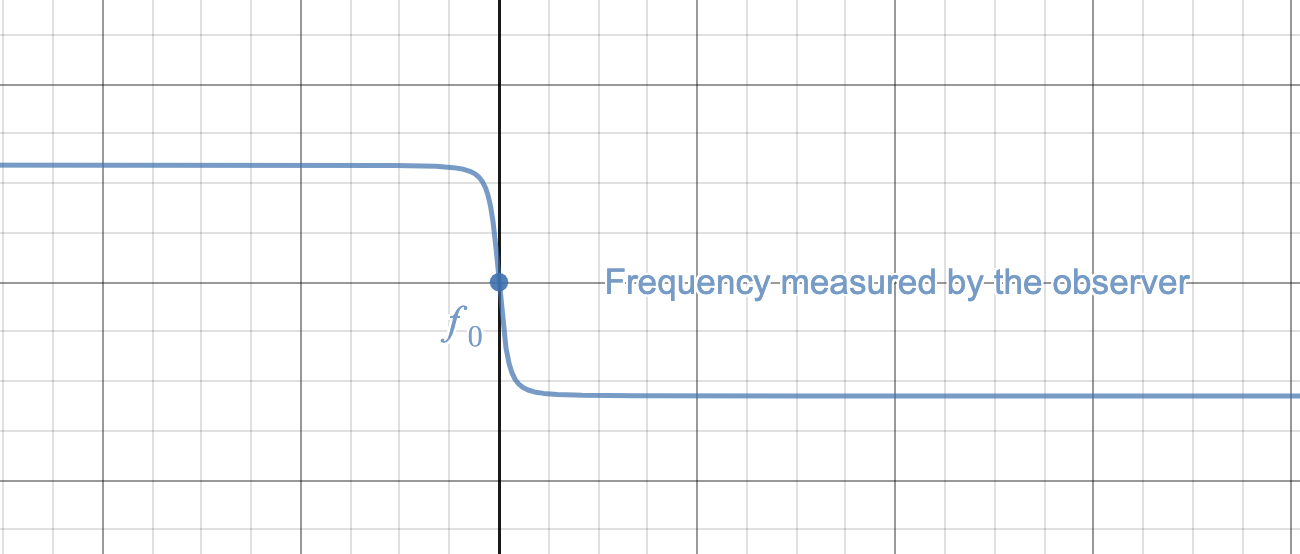
\includegraphics[width=5in]{frequency}
	\caption{Graph showing the frequency measured by the observer}
	\label{fig:frequency}
\end{figure}

\subsection{Analysis of the new formula and comparison to the old one}


\section{Sources}

Predoi, Mihai. (2014). Re: Does wavelength have an effect on sound pressure?. Retrieved from: \url{ https://www.researchgate.net/post/Does_wavelength_have_an_effect_on_sound_pressure/52c51fe9d3df3ed40f8b4610/citation/download. }

\url{https://phys.org/news/2013-02-human-fourier-uncertainty-principle.html}
\end{document}
